\documentclass[11pt,letterpaper]{article}

% Mandatory Packages
\usepackage{amsmath}
\usepackage{amssymb}
\usepackage{amsthm}
\usepackage{geometry}
\usepackage{tikz}
\usetikzlibrary{arrows.meta, positioning, shapes, backgrounds}
\usepackage{mathrsfs}
\usepackage{mathtools}
\usepackage{hyperref}
\usepackage{enumitem}
\usepackage{xcolor}

% Page Geometry
\geometry{
    top=1in,
    bottom=1in,
    left=1in,
    right=1in
}

% Theorem Environments
\theoremstyle{definition}
\newtheorem{definition}{Definition}[section]
\newtheorem{axiom}{Axiom}[section]
\newtheorem{example}{Example}[section]

\theoremstyle{plain}
\newtheorem{theorem}{Theorem}[section]
\newtheorem{lemma}[theorem]{Lemma}
\newtheorem{proposition}[theorem]{Proposition}
\newtheorem{corollary}[theorem]{Corollary}

\theoremstyle{remark}
\newtheorem{remark}{Remark}[section]

% Custom Commands
\newcommand{\E}{\mathbb{E}}
\newcommand{\V}{\mathbb{V}}
\newcommand{\R}{\mathbb{R}}
\newcommand{\N}{\mathbb{N}}
\newcommand{\Prob}{\mathbb{P}}
\newcommand{\F}{\mathcal{F}}
\newcommand{\ind}{\mathbf{1}}

\title{\textbf{Homework 3: Discrete Random Variables and Their Probability Distributions}}
\author{Tashfeen Omran}
\date{September 2026}

\begin{document}

\maketitle
\tableofcontents
\newpage

% ==========================================
% PART 1: Comprehensive Introduction
% ==========================================
\section{Part 1: Comprehensive Introduction, Context, and Prerequisites}

\subsection{Historical Context and Motivation}
The formalization of probability theory began in the 17th century through correspondence between Pierre de Fermat and Blaise Pascal regarding gambling disputes, specifically the "problem of points." However, for centuries, probability remained a collection of heuristic rules applied to combinatorial games. It was not until 1933 that Andrey Kolmogorov provided a rigorous axiomatic foundation using measure theory. The concept of a \textit{random variable} emerged as a necessary abstraction: instead of dealing with cumbersome sample spaces (like sequences of coin flips or complex physical states), mathematicians needed a way to map these abstract outcomes to the real number line, allowing the full power of real analysis and calculus to be applied to probability.

\subsection{Core Concepts \& Axioms}
To understand discrete random variables rigorously, we must first define the underlying probability space.

\begin{definition}[Probability Space]
A probability space is a triplet $(\Omega, \F, \Prob)$ where:
\begin{itemize}
    \item $\Omega$ is the \textbf{sample space} (the set of all possible outcomes).
    \item $\F$ is a \textbf{$\sigma$-algebra} on $\Omega$ (a collection of subsets of $\Omega$ containing $\Omega$, closed under complementation and countable unions). Elements of $\F$ are called \textit{events}.
    \item $\Prob: \F \to [0,1]$ is a \textbf{probability measure} satisfying Kolmogorov's Axioms: $\Prob(\Omega) = 1$, $\Prob(A) \ge 0$ for all $A \in \F$, and for any countable sequence of disjoint events $A_1, A_2, \dots$, $\Prob\left(\bigcup_{i=1}^\infty A_i\right) = \sum_{i=1}^\infty \Prob(A_i)$.
\end{itemize}
\end{definition}

\begin{definition}[Random Variable]
A random variable $Y$ is a measurable function $Y: \Omega \to \R$. This means that for any Borel set $B \subseteq \R$, the preimage $Y^{-1}(B) = \{\omega \in \Omega : Y(\omega) \in B\}$ is an event in $\F$. 
\end{definition}

\begin{definition}[Discrete Random Variable \& Probability Mass Function]
A random variable $Y$ is \textbf{discrete} if its range (image) is finite or countably infinite. Its probability distribution is completely characterized by its \textbf{Probability Mass Function (PMF)}, denoted $p(y)$, defined as:
\[ p(y) = \Prob(Y = y) = \Prob(\{\omega \in \Omega : Y(\omega) = y\}) \]
\end{definition}

\subsection{Intuition and Set-Theoretic Foundations}
Intuitively, a random variable is neither "random" nor a "variable." It is a deterministic function. The randomness comes entirely from the underlying measure $\Prob$ on $\Omega$. The random variable $Y$ acts as a lens, projecting the abstract probability mass from $\Omega$ onto the real line $\R$. This creates a \textit{pushforward measure}. The PMF $p(y)$ simply asks: "If I look at the value $y \in \R$, what is the total probability mass of all outcomes $\omega \in \Omega$ that map to $y$?"

\subsection{Key Theorems, Lemmas, and Formulas}
\begin{theorem}[Properties of a PMF]
For any discrete probability distribution, the PMF $p(y)$ must satisfy:
1. $0 \le p(y) \le 1$ for all $y$.
2. $\sum_{y} p(y) = 1$, where the sum is over all values with nonzero probability.
\end{theorem}

\begin{definition}[Expected Value]
Let $Y$ be a discrete random variable with PMF $p(y)$. The expected value (or mean) of $Y$ is:
\[ \E(Y) = \sum_{y} y p(y) \]
provided the sum is absolutely convergent ($\sum |y|p(y) < \infty$).
\end{definition}

\begin{theorem}[Law of the Unconscious Statistician - LOTUS]
If $Y$ is a discrete random variable and $g: \R \to \R$ is a real-valued function, then:
\[ \E[g(Y)] = \sum_{y} g(y) p(y) \]
\end{theorem}

\begin{definition}[Variance]
The variance of $Y$, denoted $\V(Y)$ or $\sigma^2$, measures the expected squared deviation from the mean $\mu = \E(Y)$:
\[ \V(Y) = \E[(Y - \mu)^2] \]
\end{theorem}

\begin{theorem}[Variance Shortcut Formula]
\[ \V(Y) = \E(Y^2) - [\E(Y)]^2 \]
\end{theorem}

\subsection{Prerequisites}
To master this chapter, one must be comfortable with:
\begin{itemize}
    \item \textbf{Set Theory:} Unions, intersections, complements, and partitions.
    \item \textbf{Combinatorics:} Binomial coefficients $\binom{n}{k}$, permutations, and the fundamental counting principle.
    \item \textbf{Real Analysis:} Absolute convergence of infinite series and the manipulation of double summations (Fubini-Tonelli theorem for discrete spaces).
\end{itemize}

\newpage
% ==========================================
% PART 2: Detailed Homework Solutions
% ==========================================
\section{Part 2: Detailed Homework Solutions (Rigorous Proofs \& Computations)}

\textit{Note: Per the strategic selection protocol, the following problems have been chosen to represent every distinct problem archetype found in the provided text, ensuring comprehensive mastery without redundant repetition.}

% --- Problem 3.4 ---
\subsection{Problem 3.4: Network Reliability and PMF Construction}
\textbf{Problem Statement:} Consider a system of water flowing through valves from $A$ to $B$. Valves 1, 2, and 3 operate independently, and each correctly opens on signal with probability $0.8$. Find the probability distribution for $Y$, the number of open paths from $A$ to $B$ after the signal is given. (Note that $Y$ can take on the values 0, 1, and 2.) The diagram shows Path 1 goes through Valve 1, and Path 2 goes through Valves 2 and 3 in series.

\begin{proof}[Solution]
\textbf{Step 1: Define the Probability Space and Events.}\\
Let $V_i$ be the event that Valve $i$ opens successfully, for $i \in \{1, 2, 3\}$. 
We are given $\Prob(V_i) = 0.8$ and that the events $V_1, V_2, V_3$ are mutually independent.

\textbf{Step 2: Define the Paths.}\\
Let $P_1$ be the event that Path 1 is open. Path 1 consists only of Valve 1, so $P_1 = V_1$.
Let $P_2$ be the event that Path 2 is open. Path 2 requires both Valve 2 and Valve 3 to be open, so $P_2 = V_2 \cap V_3$.
By independence, $\Prob(P_1) = \Prob(V_1) = 0.8$.
By independence, $\Prob(P_2) = \Prob(V_2 \cap V_3) = \Prob(V_2)\Prob(V_3) = (0.8)(0.8) = 0.64$.

\textbf{Step 3: Calculate the PMF for $Y$.}\\
The random variable $Y$ represents the number of open paths. Thus, $Y \in \{0, 1, 2\}$.

\textit{Case $Y = 2$ (Both paths open):}
\[ \Prob(Y = 2) = \Prob(P_1 \cap P_2) = \Prob(V_1 \cap V_2 \cap V_3) \]
By mutual independence:
\[ \Prob(Y = 2) = (0.8)(0.8)(0.8) = 0.512 \]

\textit{Case $Y = 0$ (Zero paths open):}
\[ \Prob(Y = 0) = \Prob(P_1^c \cap P_2^c) \]
Since $P_1$ depends only on $V_1$, and $P_2$ depends only on $V_2, V_3$, the events $P_1$ and $P_2$ are independent.
\[ \Prob(Y = 0) = \Prob(P_1^c) \Prob(P_2^c) = (1 - 0.8)(1 - 0.64) = (0.2)(0.36) = 0.072 \]

\textit{Case $Y = 1$ (Exactly one path open):}
Using the axiom that probabilities must sum to 1:
\[ \Prob(Y = 1) = 1 - \Prob(Y = 0) - \Prob(Y = 2) = 1 - 0.072 - 0.512 = 0.416 \]
\textit{Verification via direct computation:}
\begin{align*}
\Prob(Y = 1) &= \Prob(P_1 \cap P_2^c) + \Prob(P_1^c \cap P_2) \\
&= \Prob(P_1)\Prob(P_2^c) + \Prob(P_1^c)\Prob(P_2) \\
&= (0.8)(0.36) + (0.2)(0.64) = 0.288 + 0.128 = 0.416
\end{align*}

\textbf{Conclusion:} The probability distribution for $Y$ is:
\[ p(0) = 0.072, \quad p(1) = 0.416, \quad p(2) = 0.512 \]
\end{proof}

% --- Problem 3.6 ---
\subsection{Problem 3.6: Combinatorial PMF Construction}
\textbf{Problem Statement:} Five balls, numbered 1, 2, 3, 4, and 5, are placed in an urn. Two balls are randomly selected from the five, and their numbers noted. Find the probability distribution for the following:
(a) The largest of the two sampled numbers.
(b) The sum of the two sampled numbers.

\begin{proof}[Solution]
\textbf{Step 1: Define the Sample Space.}\\
The sample space $\Omega$ consists of all subsets of size 2 chosen from $\{1, 2, 3, 4, 5\}$. 
The total number of equally likely outcomes is $|\Omega| = \binom{5}{2} = 10$.
The outcomes are: $\{1,2\}, \{1,3\}, \{1,4\}, \{1,5\}, \{2,3\}, \{2,4\}, \{2,5\}, \{3,4\}, \{3,5\}, \{4,5\}$.

\textbf{Part (a): Let $Y_a$ be the largest of the two numbers.}\\
The possible values for $Y_a$ are $\{2, 3, 4, 5\}$. We count the number of outcomes mapping to each value:
\begin{itemize}
    \item $Y_a = 2$: Only the set $\{1,2\}$ has 2 as its maximum. (1 outcome). $p_a(2) = 1/10$.
    \item $Y_a = 3$: The sets $\{1,3\}, \{2,3\}$ have 3 as their maximum. (2 outcomes). $p_a(3) = 2/10$.
    \item $Y_a = 4$: The sets $\{1,4\}, \{2,4\}, \{3,4\}$ have 4 as their maximum. (3 outcomes). $p_a(4) = 3/10$.
    \item $Y_a = 5$: The sets $\{1,5\}, \{2,5\}, \{3,5\}, \{4,5\}$ have 5 as their maximum. (4 outcomes). $p_a(5) = 4/10$.
\end{itemize}
\textit{Check:} $1/10 + 2/10 + 3/10 + 4/10 = 10/10 = 1$.

\textbf{Part (b): Let $Y_b$ be the sum of the two numbers.}\\
The possible values for $Y_b$ range from $1+2=3$ to $4+5=9$. We map each outcome to its sum:
\begin{itemize}
    \item Sum = 3: $\{1,2\} \implies p_b(3) = 1/10$
    \item Sum = 4: $\{1,3\} \implies p_b(4) = 1/10$
    \item Sum = 5: $\{1,4\}, \{2,3\} \implies p_b(5) = 2/10$
    \item Sum = 6: $\{1,5\}, \{2,4\} \implies p_b(6) = 2/10$
    \item Sum = 7: $\{2,5\}, \{3,4\} \implies p_b(7) = 2/10$
    \item Sum = 8: $\{3,5\} \implies p_b(8) = 1/10$
    \item Sum = 9: $\{4,5\} \implies p_b(9) = 1/10$
\end{itemize}
\textit{Check:} $1+1+2+2+2+1+1 = 10$. The probabilities sum to 1.
\end{proof}

% --- Problem 3.12 ---
\subsection{Problem 3.12: Direct Computation of Expectation and Variance}
\textbf{Problem Statement:} Let $Y$ be a random variable with $p(y)$ given in the table below. Find $\E(Y)$, $\E(1/Y)$, $\E(Y^2 - 1)$, and $\V(Y)$.
\begin{center}
\begin{tabular}{c|cccc}
$y$ & 1 & 2 & 3 & 4 \\
\hline
$p(y)$ & .4 & .3 & .2 & .1
\end{tabular}
\end{center}

\begin{proof}[Solution]
\textbf{Step 1: Compute $\E(Y)$.}\\
By Definition 3.4, $\E(Y) = \sum y p(y)$:
\[ \E(Y) = (1)(0.4) + (2)(0.3) + (3)(0.2) + (4)(0.1) = 0.4 + 0.6 + 0.6 + 0.4 = 2.0 \]

\textbf{Step 2: Compute $\E(1/Y)$.}\\
By Theorem 3.2 (LOTUS), $\E[g(Y)] = \sum g(y) p(y)$ where $g(y) = 1/y$:
\begin{align*}
\E(1/Y) &= \left(\frac{1}{1}\right)(0.4) + \left(\frac{1}{2}\right)(0.3) + \left(\frac{1}{3}\right)(0.2) + \left(\frac{1}{4}\right)(0.1) \\
&= 0.4 + 0.15 + \frac{0.2}{3} + 0.025 \\
&= \frac{40}{100} + \frac{15}{100} + \frac{20}{300} + \frac{2.5}{100} = \frac{120}{300} + \frac{45}{300} + \frac{20}{300} + \frac{7.5}{300} = \frac{192.5}{300} = \frac{77}{120} \approx 0.6417
\end{align*}

\textbf{Step 3: Compute $\E(Y^2 - 1)$.}\\
By Linearity of Expectation (Theorems 3.3 and 3.5), $\E(Y^2 - 1) = \E(Y^2) - 1$.
First, compute $\E(Y^2)$:
\[ \E(Y^2) = (1^2)(0.4) + (2^2)(0.3) + (3^2)(0.2) + (4^2)(0.1) = 0.4 + 1.2 + 1.8 + 1.6 = 5.0 \]
Thus, $\E(Y^2 - 1) = 5.0 - 1.0 = 4.0$.

\textbf{Step 4: Compute $\V(Y)$.}\\
By Theorem 3.6, $\V(Y) = \E(Y^2) - [\E(Y)]^2$:
\[ \V(Y) = 5.0 - (2.0)^2 = 5.0 - 4.0 = 1.0 \]
\end{proof}

% --- Problem 3.27 ---
\subsection{Problem 3.27: Applied Expected Value (Actuarial Pricing)}
\textbf{Problem Statement:} A potential customer for an $\$85,000$ fire insurance policy possesses a home in an area that, according to experience, may sustain a total loss in a given year with probability of $.001$ and a $50\%$ loss with probability $.01$. Ignoring all other partial losses, what premium should the insurance company charge for a yearly policy in order to break even on all $\$85,000$ policies in this area?

\begin{proof}[Solution]
\textbf{Step 1: Define the Random Variable.}\\
Let $X$ be the random variable representing the payout by the insurance company in a given year.
The possible values for $X$ are:
\begin{itemize}
    \item Total loss payout: $x_1 = \$85,000$. The probability is $p(x_1) = 0.001$.
    \item $50\%$ loss payout: $x_2 = 0.5 \times 85,000 = \$42,500$. The probability is $p(x_2) = 0.01$.
    \item No loss payout: $x_3 = \$0$. The probability is $p(x_3) = 1 - 0.001 - 0.01 = 0.989$.
\end{itemize}

\textbf{Step 2: Calculate the Expected Payout.}\\
To break even, the premium charged must exactly equal the expected payout, $\E(X)$.
\begin{align*}
\E(X) &= \sum x p(x) \\
&= (85000)(0.001) + (42500)(0.01) + (0)(0.989) \\
&= 85 + 425 + 0 = 510
\end{align*}

\textbf{Conclusion:} The insurance company should charge a premium of $\$510$ to break even.
\end{proof}

% --- Problem 3.29 ---
\subsection{Problem 3.29: Theoretical Proof (Tail Sum Formula for Expectation)}
\textbf{Problem Statement:} If $Y$ is a discrete random variable that assigns positive probabilities to only the positive integers, show that
\[ \E(Y) = \sum_{k=1}^\infty \Prob(Y \ge k) \]

\begin{proof}[Solution]
\textbf{Proof Technique: Direct Proof via Interchange of Summation (Fubini-Tonelli for Discrete Measures).}\\
By definition, the expected value of $Y$ is:
\[ \E(Y) = \sum_{y=1}^\infty y p(y) \]
Notice that the integer $y$ can be written as a sum of ones: $y = \sum_{k=1}^y 1$. Substituting this into the expectation formula yields:
\[ \E(Y) = \sum_{y=1}^\infty \left( \sum_{k=1}^y 1 \right) p(y) = \sum_{y=1}^\infty \sum_{k=1}^y p(y) \]
We now have a double summation over the indices $y$ and $k$. The region of summation is defined by the inequalities:
\[ 1 \le k \le y < \infty \]
Because $p(y) \ge 0$ for all $y$, all terms in the sum are non-negative. By Tonelli's Theorem, we are permitted to change the order of summation without altering the sum's value. 
Reversing the order of summation, we first fix $k$. If $1 \le k \le y < \infty$, then for a fixed $k \ge 1$, the index $y$ must range from $k$ to $\infty$. Thus:
\[ \E(Y) = \sum_{k=1}^\infty \sum_{y=k}^\infty p(y) \]
By definition, $\sum_{y=k}^\infty p(y)$ is exactly the probability that $Y$ takes a value greater than or equal to $k$:
\[ \sum_{y=k}^\infty p(y) = \Prob(Y \ge k) \]
Substituting this back into the outer sum yields:
\[ \E(Y) = \sum_{k=1}^\infty \Prob(Y \ge k) \]
This completes the proof. $\blacksquare$
\end{proof}

% --- Problem 3.33 ---
\subsection{Problem 3.33: Theoretical Proof (Linearity of Expectation and Variance)}
\textbf{Problem Statement:} Let $Y$ be a discrete random variable with mean $\mu$ and variance $\sigma^2$. If $a$ and $b$ are constants, use Theorems 3.3 through 3.6 to prove that:
(a) $\E(aY + b) = a\E(Y) + b = a\mu + b$
(b) $\V(aY + b) = a^2 \V(Y) = a^2 \sigma^2$

\begin{proof}[Solution]
\textbf{Part (a):}\\
By Theorem 3.5 (Expectation of a sum is the sum of expectations):
\[ \E(aY + b) = \E(aY) + \E(b) \]
By Theorem 3.4 (Constants can be factored out of expectations), $\E(aY) = a\E(Y)$.
By Theorem 3.3 (The expectation of a constant is the constant), $\E(b) = b$.
Substituting these results yields:
\[ \E(aY + b) = a\E(Y) + b = a\mu + b \]

\textbf{Part (b):}\\
By Definition 3.5, the variance of a random variable $X$ is $\E[(X - \E(X))^2]$. Let $X = aY + b$.
\[ \V(aY + b) = \E\left[ \left( (aY + b) - \E(aY + b) \right)^2 \right] \]
Substitute the result from Part (a), $\E(aY + b) = a\E(Y) + b$:
\begin{align*}
\V(aY + b) &= \E\left[ \left( aY + b - a\E(Y) - b \right)^2 \right] \\
&= \E\left[ \left( aY - a\E(Y) \right)^2 \right] \\
&= \E\left[ \left( a(Y - \E(Y)) \right)^2 \right] \\
&= \E\left[ a^2 (Y - \E(Y))^2 \right]
\end{align*}
By Theorem 3.4, we can factor the constant $a^2$ out of the expectation:
\[ \V(aY + b) = a^2 \E\left[ (Y - \E(Y))^2 \right] \]
By Definition 3.5, $\E\left[ (Y - \E(Y))^2 \right] = \V(Y) = \sigma^2$. Therefore:
\[ \V(aY + b) = a^2 \V(Y) = a^2 \sigma^2 \]
This completes the proof. $\blacksquare$
\end{proof}

\newpage
% ==========================================
% PART 3: In-Depth Analysis
% ==========================================
\section{Part 3: In-Depth Analysis of Problems and Techniques}

\subsection{A) Problem Types and Logical Strategies}
The problems in this chapter fall into four distinct archetypes:
\begin{enumerate}
    \item \textbf{Combinatorial PMF Construction (e.g., 3.4, 3.6):} The strategy here is to first define the sample space $\Omega$ and calculate the probability of each atomic outcome. Then, define the mapping $Y: \Omega \to \R$. Finally, aggregate the probabilities of all outcomes that map to the same real number $y$.
    \item \textbf{Direct Expectation/Variance Computation (e.g., 3.12):} These are mechanical problems. The strategy is to strictly apply the definitions $\E(Y) = \sum y p(y)$ and LOTUS $\E[g(Y)] = \sum g(y) p(y)$. The shortcut formula $\V(Y) = \E(Y^2) - [\E(Y)]^2$ is universally preferred over the definitional formula for variance due to computational efficiency.
    \item \textbf{Applied Risk/Pricing (e.g., 3.27):} These problems require translating a real-world scenario into a random variable. The key strategy is identifying that "breaking even" or "fair value" mathematically translates to setting a fixed value equal to the Expected Value of the random payout.
    \item \textbf{Theoretical Proofs (e.g., 3.29, 3.33):} These require manipulating summations. The overarching strategy is to write out the expectation as an infinite series and apply analytical tricks (like changing the order of summation or leveraging linearity) to restructure the equation into the desired form.
\end{enumerate}

\subsection{B) Key Analytical and Logical Manipulations}
\begin{itemize}
    \item \textbf{Interchange of Summation (Fubini-Tonelli):} Used in Problem 3.29. When dealing with double sums of non-negative terms, swapping $\sum_{y=1}^\infty \sum_{k=1}^y$ to $\sum_{k=1}^\infty \sum_{y=k}^\infty$ is a powerful trick to convert an expectation into a sum of tail probabilities.
    \item \textbf{Law of Total Probability / Partitioning:} Used implicitly in Problem 3.4. To find the probability of exactly one path being open, we partitioned the event into mutually exclusive sub-events: (Path 1 open AND Path 2 closed) $\cup$ (Path 1 closed AND Path 2 open).
    \item \textbf{Linearity Extraction:} Used in Problem 3.33. The trick of expanding $(aY+b - (a\mu+b))^2$ allows the constants $b$ to cancel out, proving mathematically why shifting a distribution (adding $b$) does not change its variance (spread).
\end{itemize}

\newpage
% ==========================================
% PART 4: Cheatsheet, Visuals, and Tips
% ==========================================
\section{Part 4: "Cheatsheet", Visuals, and Tips for Success}

\subsection{Theorems \& Equivalences Summary}
\begin{itemize}
    \item \textbf{Valid PMF:} $p(y) \ge 0$ and $\sum p(y) = 1$.
    \item \textbf{Expected Value:} $\E(Y) = \sum y p(y)$.
    \item \textbf{LOTUS:} $\E[g(Y)] = \sum g(y) p(y)$.
    \item \textbf{Linearity:} $\E(aY + b) = a\E(Y) + b$.
    \item \textbf{Variance Shortcut:} $\V(Y) = \E(Y^2) - [\E(Y)]^2$.
    \item \textbf{Variance Scaling:} $\V(aY + b) = a^2 \V(Y)$.
    \item \textbf{Tail Sum (Positive Integers):} $\E(Y) = \sum_{k=1}^\infty \Prob(Y \ge k)$.
\end{itemize}

\subsection{Set \& Logic Illustration: The Random Variable Mapping}
The following TikZ diagram illustrates the rigorous measure-theoretic definition of a discrete random variable. It shows how $Y$ maps the abstract sample space $\Omega$ to the real line $\R$, and how the probability measure $\Prob$ maps those real values to the interval $[0,1]$ to create the PMF.

\vspace{0.5cm}
\begin{center}
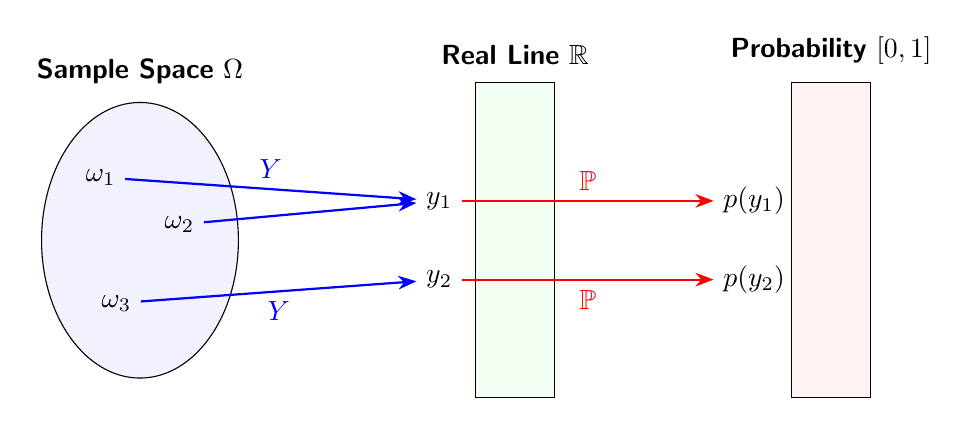
\begin{tikzpicture}[
    >=Stealth,
    node distance=3cm,
    every node/.style={font=\sffamily},
    space/.style={ellipse, draw, minimum width=2.5cm, minimum height=3.5cm, fill=blue!5},
    real/.style={rectangle, draw, minimum width=1cm, minimum height=4cm, fill=green!5},
    prob/.style={rectangle, draw, minimum width=1cm, minimum height=4cm, fill=red!5}
]

% Sample Space
\node[space] (omega) {};
\node[above=0.1cm of omega] {\textbf{Sample Space} $\Omega$};
\node (w1) at (-0.5, 0.8) {$\omega_1$};
\node (w2) at (0.5, 0.2) {$\omega_2$};
\node (w3) at (-0.3, -0.8) {$\omega_3$};

% Real Line
\node[real, right=3cm of omega] (R) {};
\node[above=0.1cm of R] {\textbf{Real Line} $\R$};
\node (y1) at (3.8, 0.5) {$y_1$};
\node (y2) at (3.8, -0.5) {$y_2$};

% Probability Interval
\node[prob, right=3cm of R] (P) {};
\node[above=0.1cm of P] {\textbf{Probability} $[0,1]$};
\node (p1) at (7.8, 0.5) {$p(y_1)$};
\node (p2) at (7.8, -0.5) {$p(y_2)$};

% Mappings Y
\draw[->, thick, blue] (w1) -- (y1) node[midway, above] {$Y$};
\draw[->, thick, blue] (w2) -- (y1);
\draw[->, thick, blue] (w3) -- (y2) node[midway, below] {$Y$};

% Mappings P
\draw[->, thick, red] (y1) -- (p1) node[midway, above] {$\Prob$};
\draw[->, thick, red] (y2) -- (p2) node[midway, below] {$\Prob$};

\end{tikzpicture}
\end{center}
\vspace{0.5cm}

\subsection{Heuristics \& "Cheats"}
\begin{itemize}
    \item \textbf{The "Sum to 1" Sanity Check:} Whenever you construct a PMF, immediately sum the probabilities. If they do not equal exactly 1, stop. You have missed an outcome or double-counted.
    \item \textbf{Variance is strictly non-negative:} If you compute $\V(Y) = \E(Y^2) - [\E(Y)]^2$ and get a negative number, you made an arithmetic error. $\E(Y^2)$ must always be $\ge [\E(Y)]^2$.
\end{itemize}

\subsection{Pitfalls \& Fallacies}
\begin{itemize}
    \item \textbf{The Non-Linearity of Functions Fallacy:} Assuming $\E[g(Y)] = g(\E[Y])$. This is almost always false unless $g$ is linear. For example, $\E(1/Y) \neq 1/\E(Y)$ (as seen in Problem 3.12) and $\E(Y^2) \neq [\E(Y)]^2$.
    \item \textbf{Confusing Independence with Mutually Exclusive:} In Problem 3.4, valves operating independently means $\Prob(A \cap B) = \Prob(A)\Prob(B)$. If they were mutually exclusive, $\Prob(A \cap B) = 0$. They are fundamentally different concepts.
\end{itemize}

\newpage
% ==========================================
% PART 5: Conceptual Synthesis
% ==========================================
\section{Part 5: Conceptual Synthesis and The "Big Picture"}

\subsection{A) Thematic Connections}
The core theme of this chapter is \textbf{measure-theoretic pushforward and aggregation}. In Chapter 2, probability was assigned to abstract sets (events). In Chapter 3, we introduce the Random Variable $Y$ to "push" that probability measure onto the real number line. This allows us to aggregate complex outcomes into numerical summaries: the Expected Value (center of mass) and Variance (moment of inertia). This unifies combinatorial probability with algebraic summation.

\subsection{B) Forward and Backward Links}
\begin{itemize}
    \item \textbf{Backward Link:} This chapter relies heavily on the axioms of probability and combinatorics established in previous chapters. The calculation of $p(y)$ is simply an application of Chapter 2 techniques to the specific event $Y^{-1}(y)$.
    \item \textbf{Forward Link:} Understanding discrete random variables is the absolute bedrock for continuous random variables (where summations become Lebesgue integrals). Furthermore, the properties of Expectation and Variance derived here are the foundation for the Central Limit Theorem, Stochastic Processes (like Markov Chains), and advanced Stochastic Calculus (where we study the evolution of random variables over time).
\end{itemize}

% ==========================================
% PART 6: Abstract Real-World Modeling
% ==========================================
\section{Part 6: Abstract Real-World Modeling (AI, ML, \& Quant Finance)}

\subsection{A) Concrete Scenarios}
1. \textbf{Statistical Learning Theory (AI/ML):} In machine learning, a model's performance is evaluated using a Loss Function $L(Y, \hat{Y})$. Because the data $Y$ is drawn from an unknown probability distribution, the loss is a random variable. The goal of ML algorithms (like Neural Networks) is Empirical Risk Minimization, which is fundamentally the optimization of the Expected Value of this discrete random variable over a training dataset.
2. \textbf{Derivative Pricing (Quant Finance):} In quantitative finance, the payoff of a discrete barrier option or a digital option depends on the path of an underlying asset. The asset's price movements can be modeled as a discrete random variable (e.g., using a Binomial Cox-Ross-Rubinstein model). The fair price of the derivative is the Expected Value of its discounted future payoff under a specific "risk-neutral" probability measure $\mathbb{Q}$.

\subsection{B) Model Problem Setup: Pricing a Credit Default Swap (CDS) Leg}
\textbf{Scenario:} We wish to model the expected payout of the default leg of a simplified Credit Default Swap. 
\textbf{State Space \& Random Variable:} Let time be discrete, $t \in \{1, 2, \dots, T\}$. Let $\tau$ be the random variable representing the time of default of a corporate bond. If the bond does not default by maturity $T$, we set $\tau = \infty$. The state space for $\tau$ is $\{1, 2, \dots, T, \infty\}$.
\textbf{Probability Measure:} Let $\mathbb{Q}$ be the risk-neutral measure. The PMF of default is $q(t) = \mathbb{Q}(\tau = t)$. The survival probability to time $t$ is $S(t) = \mathbb{Q}(\tau > t) = \sum_{k=t+1}^T q(k) + \mathbb{Q}(\tau = \infty)$.
\textbf{Mathematical Formulation:} If default occurs at time $\tau \le T$, the protection seller pays the buyer a Loss Given Default (LGD), denoted as $L$. The present value of this payout is discounted at a risk-free rate $r$. The payout function is a random variable $X$:
\[ X = \begin{cases} L \cdot e^{-r \tau} & \text{if } \tau \le T \\ 0 & \text{if } \tau = \infty \end{cases} \]
The fair value of the default leg is the Expected Value of $X$ under $\mathbb{Q}$:
\[ \E^\mathbb{Q}[X] = \sum_{t=1}^T \left( L \cdot e^{-rt} \right) q(t) \]
This demonstrates how the abstract definition of $\E[g(Y)]$ is directly used to price multi-million dollar financial instruments.

\newpage
% ==========================================
% PART 7: Common Variations and Untested Concepts
% ==========================================
\section{Part 7: Common Variations and Untested Concepts}

Based on standard advanced probability curricula, a critical concept missing from the provided homework exercises is \textbf{Jensen's Inequality for Discrete Random Variables}. While the text touches on the fact that $\E[g(Y)] \neq g(\E[Y])$ (e.g., $\E(1/Y)$ in Problem 3.12), it does not formalize the directional bound of this relationship for convex/concave functions.

\begin{theorem}[Jensen's Inequality]
Let $Y$ be a discrete random variable and let $\phi: \R \to \R$ be a convex function. Then:
\[ \phi(\E[Y]) \le \E[\phi(Y)] \]
If $\phi$ is strictly convex, equality holds if and only if $Y$ is a constant (i.e., $\Prob(Y = c) = 1$ for some $c$).
\end{theorem}

\begin{proof}[Rigorous Proof for Finite Discrete Case]
We proceed by induction on $n$, the number of values $Y$ can take.
\textbf{Base Case ($n=2$):} Let $Y$ take values $y_1, y_2$ with probabilities $p_1, p_2$ such that $p_1 + p_2 = 1$.
By the definition of a convex function, for any $t \in [0,1]$:
\[ \phi(t y_1 + (1-t) y_2) \le t \phi(y_1) + (1-t) \phi(y_2) \]
Setting $t = p_1$ and $1-t = p_2$, we get:
\[ \phi(p_1 y_1 + p_2 y_2) \le p_1 \phi(y_1) + p_2 \phi(y_2) \implies \phi(\E[Y]) \le \E[\phi(Y)] \]
\textbf{Inductive Step:} Assume the inequality holds for any random variable taking $n$ values. Let $Y$ take $n+1$ values $y_1, \dots, y_{n+1}$ with probabilities $p_1, \dots, p_{n+1}$.
\[ \E[Y] = \sum_{i=1}^{n+1} p_i y_i = p_{n+1} y_{n+1} + (1 - p_{n+1}) \sum_{i=1}^n \frac{p_i}{1 - p_{n+1}} y_i \]
Let $y^* = \sum_{i=1}^n \frac{p_i}{1 - p_{n+1}} y_i$. Note that $\frac{p_i}{1 - p_{n+1}}$ are valid probabilities summing to 1.
By convexity of $\phi$:
\[ \phi(\E[Y]) = \phi(p_{n+1} y_{n+1} + (1 - p_{n+1}) y^*) \le p_{n+1} \phi(y_{n+1}) + (1 - p_{n+1}) \phi(y^*) \]
By the inductive hypothesis applied to $y^*$:
\[ \phi(y^*) = \phi\left( \sum_{i=1}^n \frac{p_i}{1 - p_{n+1}} y_i \right) \le \sum_{i=1}^n \frac{p_i}{1 - p_{n+1}} \phi(y_i) \]
Substituting this back:
\[ \phi(\E[Y]) \le p_{n+1} \phi(y_{n+1}) + (1 - p_{n+1}) \sum_{i=1}^n \frac{p_i}{1 - p_{n+1}} \phi(y_i) = \sum_{i=1}^{n+1} p_i \phi(y_i) = \E[\phi(Y)] \]
This completes the proof. $\blacksquare$
\end{proof}

\textbf{Example Application:} In Problem 3.12, we found $\E(Y) = 2.0$ and $\E(1/Y) \approx 0.6417$. The function $\phi(y) = 1/y$ is strictly convex for $y > 0$. By Jensen's Inequality, $\phi(\E[Y]) \le \E[\phi(Y)]$. 
Indeed, $1/\E[Y] = 1/2.0 = 0.5$. And $0.5 \le 0.6417$. The inequality holds perfectly.

\newpage
% ==========================================
% PART 8: Advanced Diagnostic Testing
% ==========================================
\section{Part 8: Advanced Diagnostic Testing: "Find the Flaw"}

Below are five proofs/solutions that appear rigorous but contain a subtle, critical mathematical flaw. Your task as a grader is to identify the error. (The solutions are provided at the end of this section).

\subsection{Flawed Proof 1: The Linearity of Variance}
\textbf{Claim:} For any two discrete random variables $X$ and $Y$, $\V(X + Y) = \V(X) + \V(Y)$.
\begin{proof}
By definition, $\V(X+Y) = \E[((X+Y) - \E(X+Y))^2]$.
By linearity of expectation, $\E(X+Y) = \E(X) + \E(Y)$.
Substituting this in:
\begin{align*}
\V(X+Y) &= \E[((X - \E(X)) + (Y - \E(Y)))^2] \\
&= \E[(X - \E(X))^2 + (Y - \E(Y))^2] \\
&= \E[(X - \E(X))^2] + \E[(Y - \E(Y))^2] \\
&= \V(X) + \V(Y)
\end{align*}
Thus, variance is linear. $\blacksquare$
\end{proof}

\subsection{Flawed Proof 2: Expectation of a Ratio}
\textbf{Claim:} If $X$ and $Y$ are independent discrete random variables, then $\E[X/Y] = \E[X] / \E[Y]$.
\begin{proof}
Since $X$ and $Y$ are independent, their joint PMF factors: $p(x,y) = p_X(x)p_Y(y)$.
\begin{align*}
\E\left[\frac{X}{Y}\right] &= \sum_x \sum_y \frac{x}{y} p(x,y) \\
&= \sum_x \sum_y x \left(\frac{1}{y}\right) p_X(x) p_Y(y) \\
&= \left( \sum_x x p_X(x) \right) \left( \sum_y \frac{1}{y} p_Y(y) \right) \\
&= \E[X] \cdot \frac{1}{\E[Y]} \\
&= \frac{\E[X]}{\E[Y]}
\end{align*}
$\blacksquare$
\end{proof}

\subsection{Flawed Proof 3: The Infinite Expectation Trap}
\textbf{Claim:} Let $Y$ be a random variable taking values $y = 2^k$ with probability $p(y) = 2^{-k}$ for $k = 1, 2, 3, \dots$. The expected value $\E[Y]$ is finite and equals 0.
\begin{proof}
By definition, $\E[Y] = \sum_{k=1}^\infty y p(y) = \sum_{k=1}^\infty (2^k)(2^{-k}) = \sum_{k=1}^\infty 1$.
This is the series $1 + 1 + 1 + \dots$.
We can rewrite this series as $(1 - 1) + (1 - 1) + \dots = 0 + 0 + \dots = 0$.
Therefore, $\E[Y] = 0$. $\blacksquare$
\end{proof}

\subsection{Flawed Proof 4: Universal Tail Sum Formula}
\textbf{Claim:} For \textit{any} discrete random variable $Y$ taking integer values, $\E(Y) = \sum_{k=1}^\infty \Prob(Y \ge k)$.
\begin{proof}
Let $Y$ be a discrete random variable taking integer values.
\begin{align*}
\E(Y) &= \sum_{y=-\infty}^\infty y p(y) \\
&= \sum_{y=-\infty}^\infty \left( \sum_{k=1}^y 1 \right) p(y) \\
&= \sum_{k=1}^\infty \sum_{y=k}^\infty p(y) \\
&= \sum_{k=1}^\infty \Prob(Y \ge k)
\end{align*}
$\blacksquare$
\end{proof}

\subsection{Flawed Proof 5: Minimizing Expected Squared Error}
\textbf{Claim:} The constant $c$ that minimizes the expected squared error $f(c) = \E[(Y - c)^2]$ is the median of $Y$.
\begin{proof}
We want to minimize $f(c) = \E[(Y - c)^2]$.
Take the derivative with respect to $c$ and set it to zero:
\begin{align*}
\frac{d}{dc} \E[(Y - c)^2] &= 0 \\
\E\left[ \frac{d}{dc} (Y - c)^2 \right] &= 0 \\
\E[ -2(Y - c) ] &= 0 \\
-2\E[Y - c] &= 0 \\
\E[Y] - c &= 0 \implies c = \E[Y]
\end{align*}
Since the median is the measure of central tendency that balances the distribution, $c$ must be the median. $\blacksquare$
\end{proof}

\vspace{1cm}
\hrule
\vspace{0.5cm}
\subsubsection*{Solution Key: Finding the Flaws}
\begin{itemize}
    \item \textbf{Flaw 1:} The algebraic expansion of the square is incorrect. $(A + B)^2 = A^2 + 2AB + B^2$. The proof omitted the cross-term $2(X - \E(X))(Y - \E(Y))$. This cross-term is $2 \cdot \text{Cov}(X,Y)$. Variance is only linear if $X$ and $Y$ are uncorrelated (e.g., independent).
    \item \textbf{Flaw 2:} The error occurs in the step $\sum_y \frac{1}{y} p_Y(y) = \frac{1}{\E[Y]}$. By LOTUS, $\sum_y \frac{1}{y} p_Y(y) = \E[1/Y]$. As proven by Jensen's Inequality, $\E[1/Y] \neq 1/\E[Y]$.
    \item \textbf{Flaw 3:} The series $\sum_{k=1}^\infty 1$ diverges to $+\infty$. The manipulation $(1-1)+(1-1)$ is an invalid rearrangement of a divergent series (Grandi's series fallacy). The true expected value is infinite (this is the famous St. Petersburg Paradox).
    \item \textbf{Flaw 4:} The substitution $y = \sum_{k=1}^y 1$ is only valid if $y$ is a positive integer. If $y$ is negative, the sum $\sum_{k=1}^y 1$ is undefined or empty. The tail sum formula only works for random variables with non-negative support.
    \item \textbf{Flaw 5:} The calculus and expectation algebra are perfectly correct, proving that $c = \E[Y]$ (the Mean). The flaw is in the final concluding sentence: it falsely claims $\E[Y]$ is the Median. The mean minimizes squared error ($L_2$ loss), while the median minimizes absolute error ($L_1$ loss, $\E|Y-c|$).
\end{itemize}

\end{document}